\documentclass[a4paper,11pt]{scrartcl}
\usepackage[utf8x]{inputenc}
\usepackage[catalan]{babel}
\usepackage{titlesec}
% A ses llengües llatines, el primer paràgraf ha d'anar tabulat
\usepackage{indentfirst}
\usepackage{amsmath}
\usepackage{float}
\usepackage{graphicx}
\usepackage{subfigure}
\usepackage{booktabs}
\usepackage{multirow}
\usepackage{hyperref}
\usepackage{url}
\usepackage{multirow}
\usepackage{minted} %wget http://minted.googlecode.com/hg/minted.sty

% aptitude install texlive-fonts-extra
\usepackage{newcent} %font mes wapa

\graphicspath{{diagrames/}}

% Estil de seccions
\titleformat{\section}{\large\sectfont}{\thesection}{1em}{}
\titleformat{\subsection}{\bfseries\sectfont}{\thesubsection}{1em}{}
% Estil numeracio subseccions http://help-csli.stanford.edu/tex/latex-sections.shtml#number
%\def\thesubsection{\alph{subsection})}

\title{Robòtica: \\ Rainer\footnote{Rainer és un nom d'origen alemany i
significa guerrer decidit. També és famós ja que la muntanya Rainer és una
important fita naval d'orientació.} \ Project}
\author{ Bartomeu Miró Mateu \thanks{bartomeumiro a gmail punt com} \\
	 Lluis Cortès Rullan \thanks{lluisbinet a gmail punt com} }

\begin{document}

  \maketitle

  \begin{abstract}
    Segona pràctica de Robòtica emmarcada a l'apartat de robòtica mòbil.
    Programació d'una arquitectura de control per un robot Pioneer-3DX que
    permeti moure’s per un entorn amb obstacles i netejar un àrea mapejant
    els obstacles.
  \end{abstract}

  \newpage
  \setcounter{page}{2}
  \tableofcontents
  \newpage

  \section{Interpretació de l'enunciat}

En l'enunciat es descriu essencialment com dur a terme l'evitació d'obstacles i finalment
es proposen una sèrie de tasques a implementar com ara recorrer un conjunt de punts, vagar etc.

En aquesta pràctica s'implementa un robot netejador que vendria a ser un eufemisme per dir un
robot que intenta cobrir tots els punts d'una determinada àrea evitant els obstacles.

A banda d'aquesta funció principal també s'ha implementat la funcionalitat de vagar.

En aquesta implementació no es destaca l'originalitat de l'acció duita a terme (robot de neteja)
sinó que s'ha intentat fer èmfasi em la jerarquia de l'arquitectura i l'encapsulat de les funcions de tal
manera que un cop establert això és molt senzill desenvolupar noves tasques o afegir i modificar
funcionalitats, tema que es torna a tractar en l'apartat de possibles ampliacions.
  \section{Modelització i implementació}

\subsection{Arquitectura}
Tal i com s'explica a l'enunciat podem distingir tres nivells en l'arquitectura: estratègic, tàctic i executiu.

El nivell executiu està implementat en les llibreries de l'\emph{Aria}, així doncs la nostra pràctica implementa
els dos nivells superiors.

El nivell que més atenció requereix és el tàctic ja que l'estratègic actua com a mer seqüenciador
de funcions implementades en el tàctic.

En el codi la llibreria de l'estratègic es anomenada \texttt{librainer} i la tàctica \texttt{libtact}.

De manera transversal hi ha altres components com el mapa que el nivell tàctic omple amb les zones
per on es va passat, així com a l'estratègic per obtenir els següents punts on ordenar que vagi el robot.
Dit component apareix al codi com una llibreria anomenada \texttt{librainermap}.

També existeix una altra llibreria emprada transversalment que és \texttt{lib2d}, en aquesta s'han implementat
dues estructures de dades i les seves operacions per tal de facilitar tota la feina als demés components.
En aquesta llibreria hi trobam totes les operacions necessàries per operar amb punts i vectors bidimensionals
com ara les operacions aritmètiques clàssiques, productes per un escalar, normalitzat etc.

Finalment hi ha una llibreria no emprada al codi anomenada \texttt{libtrace} que pretenia identificar llocs
inaccessibles envoltats per objectes però finalment no s'ha acabat de implementar ja que s'ha considerat
fora de l'abast d'aquesta pràctica.


\begin{center}
  \begin{tabular}{|c|c|c|}
    \hline
    \multirow{3}{*}{lib2d} & \multicolumn{2}{|c|}{rainer}  \\
    \cline{2-3}\cline{3-3}
			  & librainer & \multirow{2}{*}{librainermap}\\
    \cline{2-2}
			  & libtact & \\
    \hline
  \end{tabular}
\end{center}


Així doncs en el nivell tàctic tenim les funcions per anar a un punt (i funcions auxiliars per el càlcul
de vectors) i la funció de vagar. Al mateix nivell s'executen dues tasques en para\lgem el una per
enregistrar els punts dels objectes trobats i una altre per enregistrar en tot moment la posició del 
robot i les zones per on ha passat marcant-les com a netes.

\subsection{Implementació de la repulsió}

En la implementació el més destacable és com es du a terme l'esquiva dels obstacles i com s'ha jugat amb
els paràmetres per evitar que el robot és bloquegi o tardi massa temps en fer un recorregut. 

El càlcul de cada un dels components és la implementació mencionada a l'enunciat, cada sensor que
detecta l'obstacle a menys d'un determinat llindar genera un vector del punt on s'ha detectat l'obstacle
al centre del robot. Aquests vectors són normalitzats, ponderats segons quin sigui el sensor i finalment
sumats.

Després és sumant ponderadament amb el vector d'atracció per tal d'obtenir la direcció resultant.

En l'elaboració del vector de repulsió es tenen amb compte tots els sensors. En principi es podria pensar
que basten els de davant ja que són els que detecten l'objecte, però es interessant posar els de darrera
ja que en el moment que intenta fer l'esquiva els de davant perden la lectura mentre que els de darrera
la guanyen i així s'afavoreix un distanciament més ràpid i perpendicular de l'objecte. 

La ponderació de cada un dels vectors s'ha fet de manera experimental amb el simulador, es pot dir
que els frontals tenen més rellevància que els de darrera, i que les diagonals tenen també major
ponderació ja que s'ha observat que així s'esquiven millor els cantons prims com per exemple d'un triangle.

El problema de l'esquiva d'un obstacle pot ser que els vectors quedin igualats i el robot bloquejat
o fent uns petits moviments ja que no te temps avançar perquè a l'haver-se re-orientat no detecta l'obstacle
i intenta tornar al punt d'on venia perquè és més proper a l'objectiu. Per això s'implementa un temps de
ceguera (\emph{blindTime}) que el robot no mira els sensors i es mou en la direcció prèviament calculada.
D'aquesta manera quan el robot s'apropa a un obstacle i la repulsió es suficient aquest es gira en sentit
oposat i avança.

Per altra banda es permet que el robot avanci mentre gira cosa que no sols agilitza el moviment sinó que
modifica la trajectòria del robot evitant que torni al mateix punt disminuint les possibilitats de bloqueig.

Cal esmentar que això no garanteix que es pugui esquivar qualsevol obstacle per arribar a un punt, 
si l'obstacle es suficientment gran és possible que el robot vagi de banda a banda d'aquest de manera
cíclica sense aconseguir superar-lo. En la secció d'ampliacions es comenta una possible so\lgem ució. En
la secció següent s'expliquen els paràmetres que governen aquest comportament, que són el temps
de ceguesa i el llindar que considera que el robot ja esta orientat per poder moure's.

\subsection{Implementació del vagar}

La implementació del vagar consisteix en avançar fins a trobar un obstacle i un cop es té posar 
la nova direcció del robot com el vector de repulsió generat per aquest obstacle.

\subsection{Implementació de la zona de neteja}

Finalment comentar que per tal de simplificar l'entorn és modelitza la zona a netejar com una retícula
de ce\lgem d'igual dimensió caracteritzades per les coordenades del seu centre i l'estat en que es troben,
si netes, brutes o son una zona ocupada per un obstacle.

En la implementació trobam que el robot comença la neteja d'una zona, la ce\lgem a a netejar és simplement
el resultat de fer un zig-zag per tota la zona, independentment si esta neta o no. Alhora hi ha dues tasques
iniciades que van registrat per on ha passat el robot i per tant consideren que s'ha netejat la zona, l'altra
observa els valors dels sensors per la detecció d'obstacles. Cal dir que aquesta segona sols mira els sensors,
no fa res més, aquest fet està comentat a l'apartat de possibles ampliacions.

Els obstacles es marquen a nivell estratègic quan el nivell tàctic indica que no ha pogut arribar a aquell
punt perquè coincideix amb un objecte. El fet de no fer-ho dins la tasca de mapeig és perquè un obstacle
pot ser suficientment petit com per representar un problema a l'aproximació des de un sol costat, així doncs
si es fa a nivell de la funcióe \emph{anar a punt} del tàctic aquesta l'intenta vorejar amb l'evitació d'obstacles, 
si en canvi es marques amb la simple tasca de detecció ja es consideraria una ce\lgema amb obstacle i s'aniria a la següent.

Un cop s'ha fet tot el zig-zag es marquen per tal de comprovar si els obstacles no eren transitoris es marquen
com ce\lgem brutes \ref{neteja} i és cerca la més propera al robot, aquest intenta accedir-hi i determina si l'ha netejat o es definitivament un
obstacle\ref{netejaobs}. Tot seguit cerca el següent punt més proper per dur a terme el mateix proces fins a donar per verificats tots els punts.

 
  \section{Explicació de paràmetres}

Tota la practica ve parametritzada per el fitxer config.cfg.

Per tal d'entendre els paràmetres on a continuació s'expliquen.

\begin{description}
  \item[thHeading] És el llindar passat a la funció que orienta el robot el qual marca si ja es considera orientat.
Aquest valor es emprat per fer les orientacions més precises quan no es vol que es mogui el robot mentre es fa el gir.
  \item[thObsHeading] A l'igual que l'anterior però aquest cop el llindar és molt permissiu, permetent que el robot
es consideri orientat i per tant segueixi avançant mentre acaba l'orientació. Sol emprar-se quan es fa l'esquiva
d'un objecte per els motius explicats en la secció anterior.

  \item[thOnPoint] És el llindar per considerar que el robot ja es troba al punt indicat, significa que la distància
entre la posició actual del robot i punt de destí ha des ser menor a aquest llindar per considerar que ja s'ha arribat.
  \item[maxDist] Es la distància a la qual un objecte es considera obstacle i per tant s'inicia la repulsió.
  \item[impactDist] Distància a la qual un objecte es considera massa proper al robot i que per tant s'ha
d'actuar de manera imminent per evitar una co\lgem isió sols tenint amb compte el vector de repulsió.
  \item[timeObstacledTh, distObstacledTh, elephantMem] Paràmetres per la llibreria \texttt{libtact} no acabada d'implementar.
  \item[blindTime] Temps entre mesures dels sensors, durant aquest temps el robot segueix l'ultima direcció donada.
  \item[numSonar] Número total de sensors a tenir amb compte.
  \item[numFirstSonar] Posició del primer sensor.
  \item[numLastFrontSonar] Posició de l'últim sensor frontal.
  \item[numLastSonar] Posició de l'últim sensor.
  \item[weightGoalAttraction] Ponderació del vector d'atracció del lloc on es vol anar.
  \item[weightObstacleRepulsion] Ponderació del vector de repulsió.
  \item[slowVel] Velocitat lenta del robot per dur a terme accions o aproximacions perilloses.
  \item[normalVel] Velocitat normal del moviment del robot.
  \item[weightSonar\#] Ponderació de cada un dels sensors del robot.
  \item[cellEdge] Dimenció de l'aresta de cada ce\lgem del mapa
  \item[area\#size] Dimensions en ce\lgem es de l'area a netejar per el robot.
  \item[robot\#init] Ce\lgem a inicial on el robot està hubicat.
\end{description}

  \section{Joc de proves}

Per tal de provar la pràctica s'han realitzat una sèrie de jocs de proves
descrits a continuació. Per cada un d'ells s'ha generat un mapa amb el
\emph{Mapper3Basic} i es poden trobar a la carpeta \emph{maps}.

Al \texttt{Makefile} es troben totes les opcions comentades a l'apartat \emph{sim}, així doncs
es descomenta la desitjada i es comenta la que està per defecte. A continuació
es canvia el codi font
de \texttt{rainer.cpp} comentant el cleanArea i descomentant l'opció desitjada.
Un cop fet això amb un \emph{make} és compila el codi i amb el \emph{make sim}
s'executa el simulador.

El primer test és simple, \textbf{passar per quatre punts sense cap obstacle}. Amb aquest simplement es comprova que es calculi
bé el vector d'atracció. També es pot observar si el \emph{heading} es fa de
manera adequada. Per fer aquesta execució no s'empre cap mapa.

\begin{figure}[H]
\begin{center}\label{4punts}
 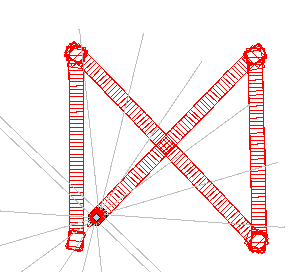
\includegraphics[width=0.5\textwidth]{diagrames/figures/4punts.png}
 % ordreRotacions.png: 1286x768 pixel, 150dpi, 21.77x13.00 cm, bb=0 0 617 369
\end{center}
  \caption{Quatre puts sense obstacle}
\end{figure}

En segon lloc tenim \textbf{passar per quatre punts però amb un obstacle}
enmig. En aquest es veu si l'esquiva d'obstacles es fa bé. A més l'obstacle està
co\lgem ocat de tal manera que el robot es troba impactant una línia de 45 graus
amb el punt destí a la perpendicular, de tal manera que seria una situació
delicada on quedar-se estancat. Per fer aquesta execució s'empra el mapa
\emph{obstacleInclinat}.

\begin{figure}[H]
\begin{center}\label{4puntsObs}
 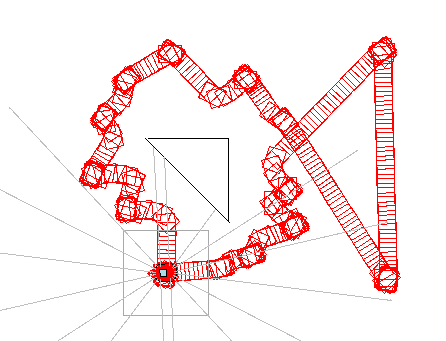
\includegraphics[width=0.5\textwidth]{diagrames/figures/4puntsObs.png}
 % ordreRotacions.png: 1286x768 pixel, 150dpi, 21.77x13.00 cm, bb=0 0 617 369
\end{center}
  \caption{Quatre puts sense obstacle}
\end{figure}

A continuació trobam el mateix \textbf{obstacle} però aquest cop \textbf{situat sobre el punt de destí}, en aquest cas
el robot ha de detectar que no pot arribar-hi ja que l'obstacle i el punt de
destí estan per davall d'un cert llindar. Fins que no s'assoleix aquest llindar
es veu com el robot intenta fer aproximacions al punt desde diferents
direccions. En aquest test empram el mapa \emph{obstacleApunt}.

\begin{figure}[H]
\begin{center}\label{obsapunt}
 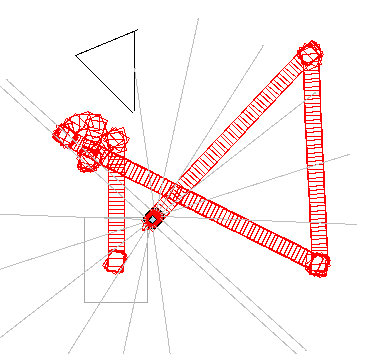
\includegraphics[width=0.5\textwidth]{diagrames/figures/obsapunt.png}
 % ordreRotacions.png: 1286x768 pixel, 150dpi, 21.77x13.00 cm, bb=0 0 617 369
\end{center}
  \caption{Quatre puts sense obstacle}
\end{figure}

Per tal de provar el \textbf{vagar} tenim un mapa tancat amb diversos obstacles
on el robot va rebotant.
Pot arribar un punt en que el robot entri en un cicle ja que els angles de rebot
poden fer que així coincideixi. El que no es permet es que el robot toqui un
obstacle o es quedi immòbil sols girant sobre ell mateix sense ser capaç de
emprendre la ruta cap a una altra banda.

\begin{figure}[H]
\begin{center}\label{vagant}
 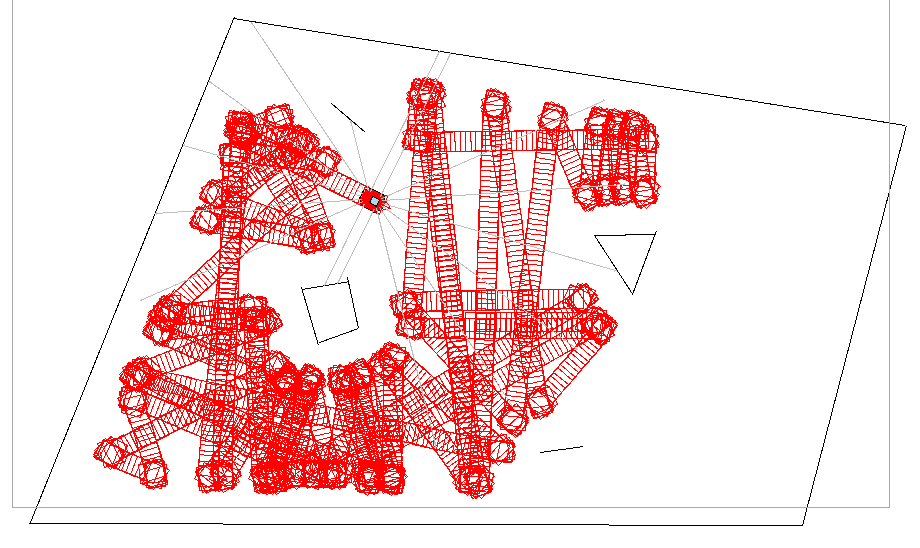
\includegraphics[width=0.5\textwidth]{diagrames/figures/vagant.png}
 % ordreRotacions.png: 1286x768 pixel, 150dpi, 21.77x13.00 cm, bb=0 0 617 369
\end{center}
  \caption{Quatre puts sense obstacle}
\end{figure}

A continuació tenim les proves de la \textbf{neteja de zona}, la primera \textbf{sense obstacles} per veure el recorregut.

\begin{figure}[H]
\begin{center}\label{neteja}
 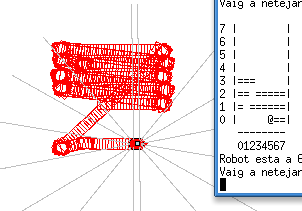
\includegraphics[width=0.5\textwidth]{diagrames/figures/netNoObs.png}
 % ordreRotacions.png: 1286x768 pixel, 150dpi, 21.77x13.00 cm, bb=0 0 617 369
\end{center}
  \caption{Quatre puts sense obstacle}
\end{figure}

I finalment la \textbf{neteja amb obstacles} on el robot els esquiva (i marca terreny durant aquesta esquiva)
i com finalment torna a les zones d'obstacle per comprovar que no fos un
obstacle mòbil i ara si que pot netejar la zona. En aquest últim no podem
simular obstacles mòbils però si veure com torna a intentar anar a la zona
obstaculitzada.

\begin{figure}[H]
\begin{center}\label{netejaobs}
 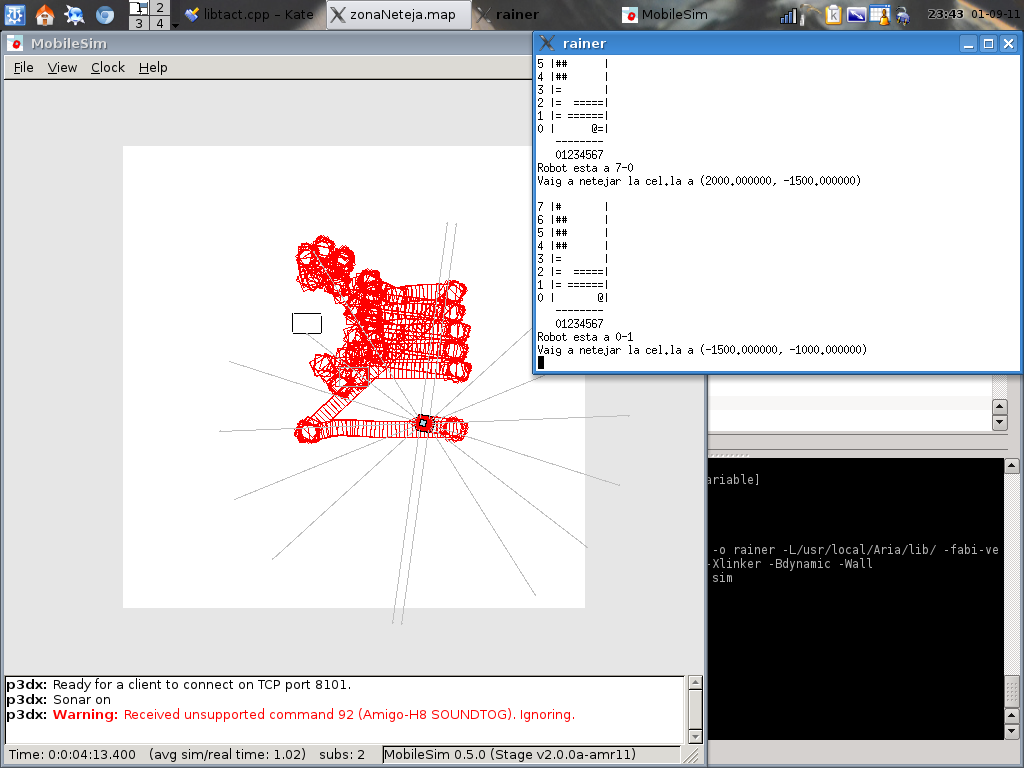
\includegraphics[width=0.5\textwidth]{diagrames/figures/netejant.png}
 % ordreRotacions.png: 1286x768 pixel, 150dpi, 21.77x13.00 cm, bb=0 0 617 369
\end{center}
  \caption{Primera passada de la neteja}
\end{figure}

\begin{figure}[H]
\begin{center}\label{figescenari}
 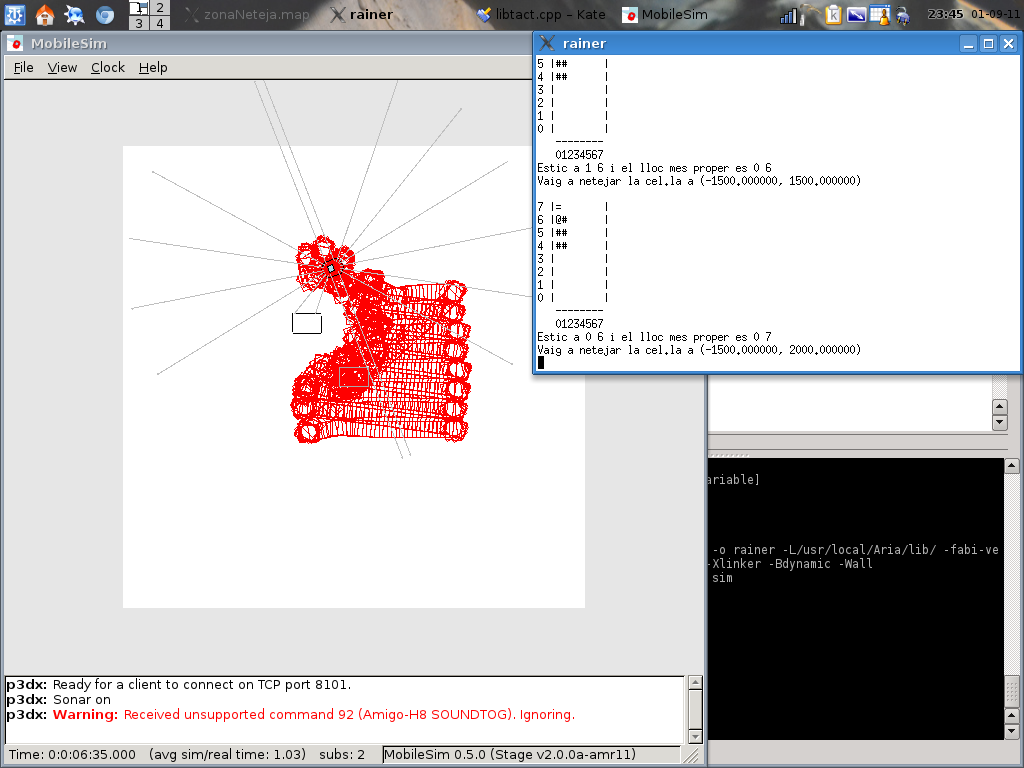
\includegraphics[width=0.5\textwidth]{diagrames/figures/netejant-aobstacles.png}
 % ordreRotacions.png: 1286x768 pixel, 150dpi, 21.77x13.00 cm, bb=0 0 617 369
\end{center}
  \caption{Segona passada de la neteja anant als punts detectats com obstacle}
\end{figure}


  \section{Possibles ampliacions}

En aquest apartat es mencionen possibles ampliacions de la pràctica actual. El fet de fer aquestes mencions
és perquè així es demostra la flexibilitat de l'arquitectura implementada i alhora mostra el grau
de comprensió adquirit veient com es podria continuar treballant.

El fet de no implementar aquestes ampliacions es perquè és costós en temps per els pocs coneixements
que es demostren.

\subsection{Ruta de neteja òptima}
Una primera millora seria implementar un viatjant de comerç per passar a fer la neteja de tots els punts.
Per fer això simplement seria necessari implementar la funció que generés la ruta òptima, guardar-la en 
memòria i implementar un iterador perquè cada crida de la funció \texttt{getNextCell} recorrér el punt on s'ha d'anar.
Dit iterador es una simple vector amb un punter també conegut com \emph{array vulgaris}.
Amb aquesta implementació s'evitarien recorregunts innecessaris sobre ce\lgem es ja netejades i el recorregut
mínim per fer-ho.

Hem de tenir amb compte que el cost és NP i el fet de trobar un obstacle pot esgarrar fàcilment la ruta.

\subsection{Atenció d'emergències}
Per altra banda seria senzill implementar una espera d'esdeveniments de teclat perquè el robot atengui una urgència,
simplement podria fer-se amb una tasca nova pendent d'esdeveniments de teclat que sobreescrigui el valor del  punt
on ha d'anar el robot.

Notem que com que la tasca de posicionar el robot al mapa i de mirar que s'ha netejat són una tasca apartat
a l'atendre una emergència també es considerarien nets els punts per on ha passat per atendre-la.

\subsection{Inaccessibilitat}
Finalment també es podria treballar el fet de trobar llocs inaccessibles. Una opció per fer-ho
es un cop iniciat el moviment a un punt guardar en un vector els punts per on es passa i quan passa
cert llindar de temps mirar si la posició actual es un punt ja dins del vector, així podríem comprovar
si està movent-se de costat a costat intentant accedir a un lloc on no es possible.

Dita funcionalitat sol requereix una lleu modificació a la tasca que registra els punts per on s'està
passat i una variable de comunicació.

\subsection{Imatge del mapa}

Finalment també seria interessant que la tasca que vigila el valors dels sensors escrivís a un mapa de bits
les lectures fetes, així es tindria una imatge amb el mapa de la situació. Aquesta funcionalitat 
en l'estat actual de la pràctica és molt senzilla de implementar, però requereix tenir soltura emprant
mapes de bits i generant imatges.

A l'igual que l'anterior seria una modificació a la tasca que registra els punts per on s'està passant.
  \emph{Valoració}

La practica ha resultat molt interessant, al principi va costar un poc adequar l'entorn de treball.
Per tal de poder emprar la llibreria i el simulador \emph{MobileSim} en la \emph{Debian} que empram normalment
va requerir compilar-ho de nou cosa que generà algun problema de dependències però va quedar sobradament
compensat per la comoditat de no haver de emprar una màquina virtual.

Cal destacar que el \emph{Mapper3Basic} i el \emph{MobileSim} són de gran ajuda a l'alumne i permeten fer simulacions
per res comparables amb la primera pràctica del braç robot que resulten vitals per el desenvolupament de la pràctica.

La llibreria \emph{Aria} en general esta força bé i és bastant intuïtiva, rara vegada s'ha hagut de cercar
informació addicional que no figurés a la API.

Per altra banda s'ha de mencionar que el \emph{C++} ens ha suposat algun mal de cap, sobretot en l'àmbit
de visibilitat dels procediments i l'ús de punters. En aquest sentit ens hagués agradat tenir temps
per provar de fer la pràctica amb \emph{Python} ja que l'\emph{Aria} en te uns \emph{bindings}. 
L'únic fet que ens tirà endarrere es que no sabíem si funcionaria
el simulador i que possiblement la llibreria no està insta\lgem al robot real.

També ens han portat molts mal de cap el trobar valors adequats per cada una de les ponderacions i llindars,
sovint ens trobàvem que amb certa combinació de llindars, especialment als de \emph{heading} el robot podia quedar
fent voltes sobre si mateix si el punt on havia d'anar era proper al punt actual però havia de fer un canvi
d'orientació. 

\begin{figure}[H]
\begin{center}\label{headingthproblem}
 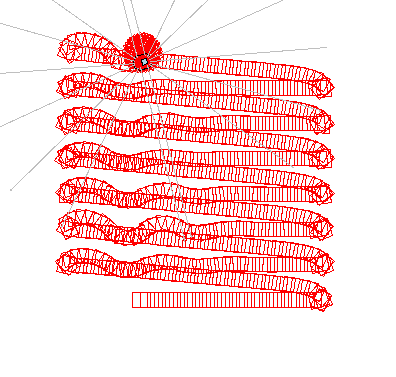
\includegraphics[width=0.5\textwidth]{diagrames/figures/voltes.png}
 % ordreRotacions.png: 1286x768 pixel, 150dpi, 21.77x13.00 cm, bb=0 0 617 369
\end{center}
  \caption{Problema amb llindar de heading}
\end{figure}

Atribuirem aquest problema a que el robot inicia el moviment abans d'estar orientat però donat que la
proximitat es molt gran no acaba d'orientar-se mai.


Tot i així i encara que ens hagués agradat implementar alguna cosa més consideram la pràctica acabada
i assolits els coneixements bàsics i que per tant les implementacions que tenim en ment i figuren en l'apartat
d'ampliacions es converteien en rutina ja que no requereixen conceptes nous sinó simples combinacions i modificacions 
sobre l'arquitectura i rutines ja implementats. %% De la practica i tecnologia emprara en si i tamb e de contingut
   \let\thefootnote\relax\footnotetext{
 Aquest document està baix llicència \href{http://creativecommons.org/licenses/by-sa/3.0/}{Creative Commons Atributive Share-Alike 3.0}
 per tant es pot compartir, modificar i distribuir, però citant els autors originals i sense modificar la llicència.
 De la mateixa manera el codi font està baix llicència GNU GPL v3 per part dels dos autors.\bigskip}
\let\thefootnote\relax\footnotetext{El document en versió digital i el codi font el trobareu a \\
\url{https://github.com/bmiro/rainer}\bigskip}
\let\thefootnote\relax\footnotetext{Aquest document i tota la part de la practica que s'ha pogut ha estat desenvolupat emprant programari lliure:}
\let\thefootnote\relax\footnotetext{\href{http://www.tug.org/applications/pdftex/}{\LaTeX} i \href{http://www.tug.org/applications/pdftex/}{Kile} per el text,
\href{http://www.inkscape.org/}{Inkscape} pels diagrames,
\href{http://kate-editor.org/}{Kate} i \href{http://vim.org/}{Vim} per l'edició del codi font.
\href{http://git-scm.com/}{Git} com a sistema de control de versions.
}

\let\thefootnote\relax\footnotetext{
\begin{center}
\begin{tabular}{cc}

\includegraphics[height=35pt,keepaspectratio=true]{diagrames/by-sa.png}
 & 
\includegraphics[height=35pt,keepaspectratio=true]{diagrames/gnu.png}
\end{tabular}
\end{center}
\begin{center}
\begin{tabular}{cccccc}
 
\includegraphics[height=35pt,keepaspectratio=true]{diagrames/latex.png}
 & 
\includegraphics[height=35pt,keepaspectratio=true]{diagrames/kile.png}
 & 
\includegraphics[height=35pt,keepaspectratio=true]{diagrames/inkscape.png}
 & 
\includegraphics[height=35pt,keepaspectratio=true]{diagrames/kde.png}
 & 
\includegraphics[height=35pt,keepaspectratio=true]{diagrames/vim.jpg}
 & 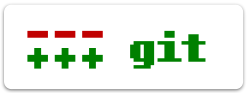
\includegraphics[height=35pt,keepaspectratio=true]{diagrames/git.png}
\end{tabular}
\end{center}
}

  \section{Annex: Codi font complet}

\subsection{Rainer, cos principal}
\inputminted[linenos, frame=lines, fontsize=\footnotesize]{cpp}{../rainer.cpp}
\newpage
\subsection{librainer, llibreria de l'estratègic}
\inputminted[linenos, frame=lines, fontsize=\footnotesize]{cpp}{../librainer.h}
\inputminted[linenos, frame=lines, fontsize=\footnotesize]{cpp}{../librainer.cpp}
\newpage
\subsection{libtact, llibreria del nivell tàctic}
\inputminted[linenos, frame=lines, fontsize=\footnotesize]{cpp}{../libtact.h}
\inputminted[linenos, frame=lines, fontsize=\footnotesize]{cpp}{../libtact.cpp}
\newpage
\subsection{librainermap, llibreria transversal del mapa}
\inputminted[linenos, frame=lines, fontsize=\footnotesize]{cpp}{../librainermap.h}
\inputminted[linenos, frame=lines, fontsize=\footnotesize]{cpp}{../librainermap.cpp}
\newpage
\subsection{lib2d, llibreria transversal d'aritmètica de vectors i punts}
\inputminted[linenos, frame=lines, fontsize=\footnotesize]{cpp}{../lib2d.h}
\inputminted[linenos, frame=lines, fontsize=\footnotesize]{cpp}{../lib2d.cpp}

\end{document}
